% !TEX encoding = UTF-8
% !TEX TS-program = pdflatex
% !TEX root = ../tesi.tex

%**************************************************************
\chapter{Progetto di stage}
\label{cap:progetto-stage}

L'azienda \azienda{} ha da sempre mostrato interesse nell'inserimento all'interno del contesto aziendale di stagisti, studenti o altre figure professionali, anche per limitati periodi di tempo. Questa particolare propensione permette all'azienda sia di promuovere nuovi progetti o attività, che con il personale a disposizione non sarebbero percorribili per questioni di tempo, sia introdurre idee e tecnologie innovative per futuri prodotti o per quelli già sviluppati ed utilizzati da \azienda{}.\\ 

\section{Descrizione del progetto}
Negli ultimi anni \azienda{} si è interessata allo creazione e sviluppo di \gls{chatbot} per Facebook Messenger, dando la possibilità ai clienti di richiederne lo sviluppo di nuovi secondo le proprie specifiche, oppure di creare il proprio \gls{chatbot} autonomamente, senza alcuna conoscenza tecnica, attraverso dei template ottimizzati per i più comuni modelli di business.\\
Il progetto di stage si inserisce in questo ambito, in quanto l'azienda desiderava introdurre la possibilità per gli utenti di scrivere delle vere e proprie domande al \gls{chatbot}, senza dover utilizzare il menù o i pulsanti dei vari modelli che la piattaforma mette a disposizione.
\begin{figure}[h]
	\centering
	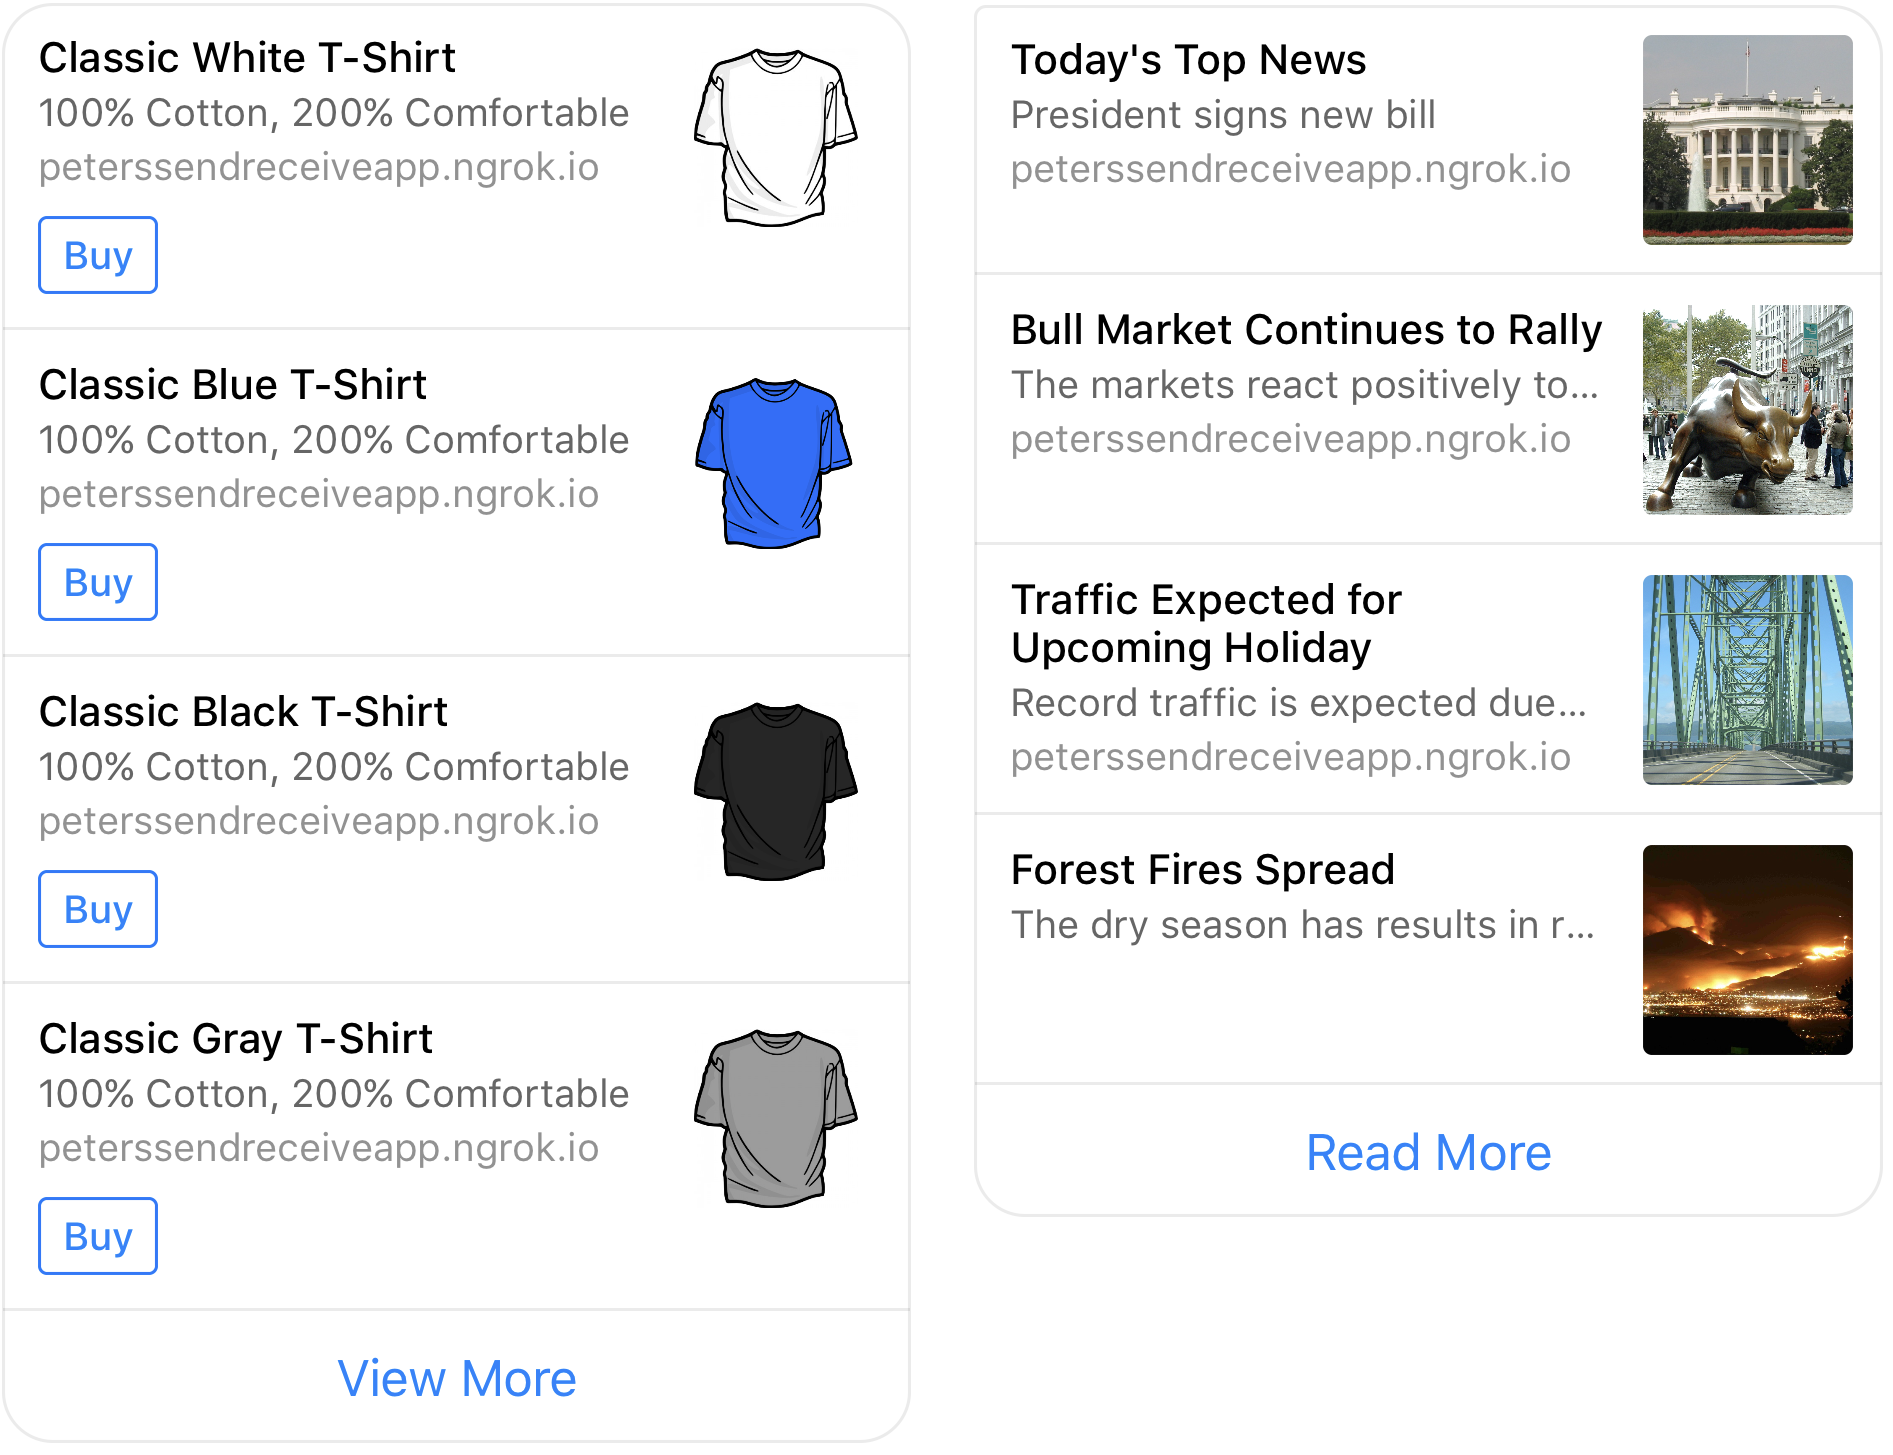
\includegraphics[scale=0.2]{../Immagini/modello_lista.png}
	\caption{Modello generico di carosello per Facebook Messenger}
\end{figure}
\newpage
Il compito assegnato allo stagista è stato quello di integrare questo meccanismo in due diversi \gls{chatbot} creati dall'azienda:
\begin{itemize}
	\item \textbf{gestore eventi}: è un applicativo creato da \azienda{} per essere utilizzato durante lo svolgimento di eventi della durata di uno o più giornate. Attraverso questo \gls{chatbot} l'utente può recuperare delle informazione riguardanti le conferenze in programma, le aule disponibili e le giornate dell'evento;
	\item \textbf{meteo Veneto bot}\footcite{meteo} questo \gls{chatbot} utilizza i dati di ARPA Veneto\footcite{arpav} per mostrare le previsioni del tempo del Veneto;
\end{itemize}
Il progetto si divideva quindi in tre parti:
\begin{itemize}
	\item analisi preliminare degli SDK delle principali piattaforme per il \gls{nlp} presenti sul mercato, in modo da valutarne pregi e difetti;
	\item creazione della logica per la gestione delle domande utente all'interno della piattaforma scelta;
	\item integrazione di questa nuova funzionalità nel software utilizzato da \azienda{} per la gestione dei \gls{chatbot}. 
\end{itemize}
Visto il bisogno di un periodo iniziale di studio, sia per capire le possibilità e i limiti degli strumenti da dover utilizzare nella trasformazione delle FAQ in dati processabili, sia per apprenderne a pieno il funzionamento tramite la documentazione presente, \azienda{} ha ritenuto questo progetto idoneo ad uno studente universitario, il quale ha a disposizione circa 300 ore per formarsi su tutto ciò di cui vi è bisogno, e successivamente portare a termine il prodotto richiesto.
\section{Principali problematiche}
sdfgsdg
\section{Strumenti utilizzati}
\subsection{NetBeans}
NetBeans è un ambiente di sviluppo integrato multi-linguaggio, nato nel giugno 2000 e scritto interamente in Java, scelto dalla Oracle Corporation come IDE ufficiale da contrapporre al più diffuso Eclipse.
L'azienda non ha posto nessun vincolo sull'ambiente di sviluppo da adottare, così come vale per i propri dipendenti. Ho deciso di utilizzare NetBeans in quanto è molto intuitivo e di semplice utilizzo.
\begin{figure}[h]
	\centering
	
\includegraphics[scale=0.4]{../Immagini/netbeans.jpg}
	\caption{Logo di NetBeans}
\end{figure}
\subsection{Api.ai}
Api.ai è una società nata nell'ottobre del 2010 e acquisita da Google Inc. nel 2016. Api.ai è una piattaforma di conversazione
che permette interazioni sofisticate con il linguaggio naturale. All'interno del progetto è stata utilizzata per trasformare le domande degli utenti in dati processabili, dopo aver creato due agenti, uno per ciascun \gls{chatbot}, ed averli istruiti secondo le possibili FAQ dei rispettivi ambiti di utilizzo.
\begin{figure}[!h]
	\centering
	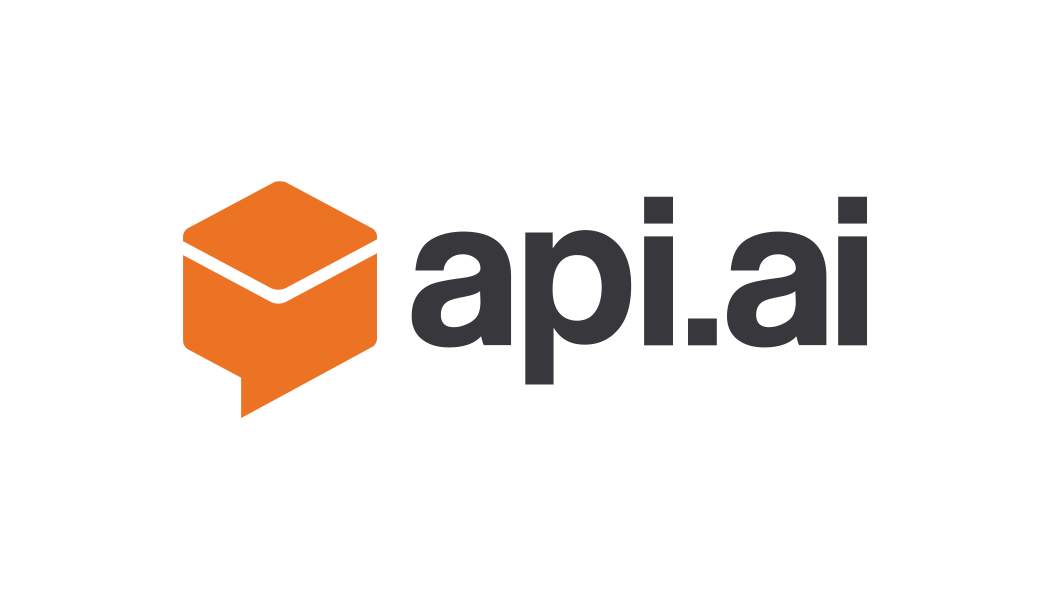
\includegraphics[scale=0.2]{../Immagini/apiai.png}
	\caption{Logo di api.ai}
\end{figure}
\subsection{Hibernate}
Hibernate è una piattaforma open-source ad alto rendimento per lo sviluppo di applicazioni Java, che fornisce il servizio Object-relation mapping (ORM), ovvero si occupa della mappatura tra le classi Java e le relative tabelle di un database SQL.
Gestisce dunque il salvataggio degli oggetti di tali classi ed il reperimento dalle entità dal database, automatizzando le query necessarie e provvedendo alla reistanziazione dell’oggetto mappato sul database.
\begin{figure}[!h]
	\centering
	
\includegraphics[scale=0.35]{../Immagini/Hibernate.png}
	\caption{Logo di Hibernate}
\end{figure}
\subsection{Apache Tomcat}
\subsection{Spring}
\subsection{Mercurial}

\subsection{BitBucket}
\section{Prodotto ottenuto}

dgsdg
